%!TEX root = ../3dbook.tex
% chktex-file 46
% chktex-file 36

\setchapterpreamble[u]{\margintoc}

\graphicspath{{conversion/}}
% \renewcommand*{\thelesson}{6.2}

\chapter{Conversions between 3D representations and formats}%
\label{chap:conversion}

% This chapter describes different conversions between 3D representations and formats that a geomatics engineer might have to perform.
% It does not claim to be an overview of all potential conversions, but it rather offers insights about the algorithms and methods most commonly used, and points out pitfalls to be aware of.

% %% to dmds

% The chapter is divided into two distinct parts:
% \begin{description}
%   \item[Fields:] conversions that are performed when we are dealing with a \emph{field}, let it be the temperature or the concentration of a certain chemical in the air (modelled as a 3D volume).
%   We name such field a trivariate field: each location ($x,y,z$) in space has one attribute.%
%   \index{trivariate field}\marginnote{trivariate field}
%   Voxels are usually what is used to represent, exchange, and analyse fields in 3D.%
%   \index{voxels}\marginnote{voxels}
%   \item[Objects:] when we are dealing with data (points, surfaces, and volumes) that represent the boundaries of objects in our environment. 
%   These can be sample points from lidar or dense matching of images, or the b-rep of some buildings (which have been reconstructed with different acquisition methods).%
%   \index{b-rep}\marginnote{boundary representation (b-rep)}
% \end{description}

%%% to dmds
%
\section{Conversions for fields}

%%%
\subsection{Conversion to isosurfaces}

Given a trivariate field $f(x,y,z) = a$, an isosurface is the set of points in space where $f(x,y,z) = a_0$, where $a_0$ is a constant. 
Isosurfaces, also called \emph{level sets}, 
\marginnote{isosurfaces, or level sets}
are the three-dimensional analogous concept to isolines (also called contour lines), which have been traditionally used to represent the elevation in topographic maps.
% Figure~\ref{fig:isosurface} shows one concrete example.
% \begin{figure*}
%   \centering
%   \begin{subfigure}[b]{0.3\linewidth}
%     \centering
%     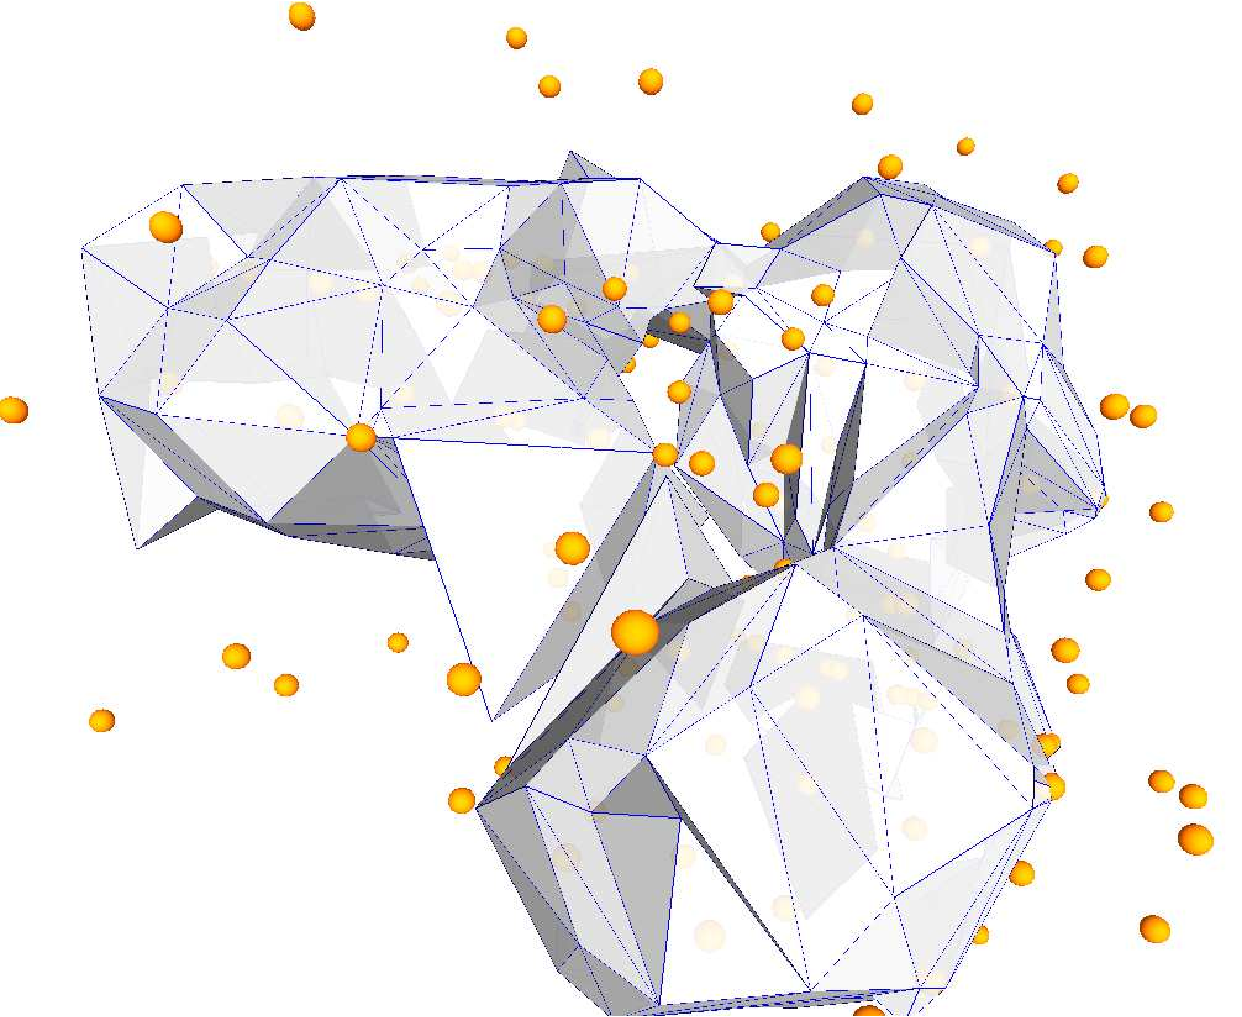
\includegraphics[width=\textwidth]{figs/isosurface2}
%     \caption{}
%   \end{subfigure}%
%   \quad
%   \begin{subfigure}[b]{0.3\linewidth}
%     \centering
%     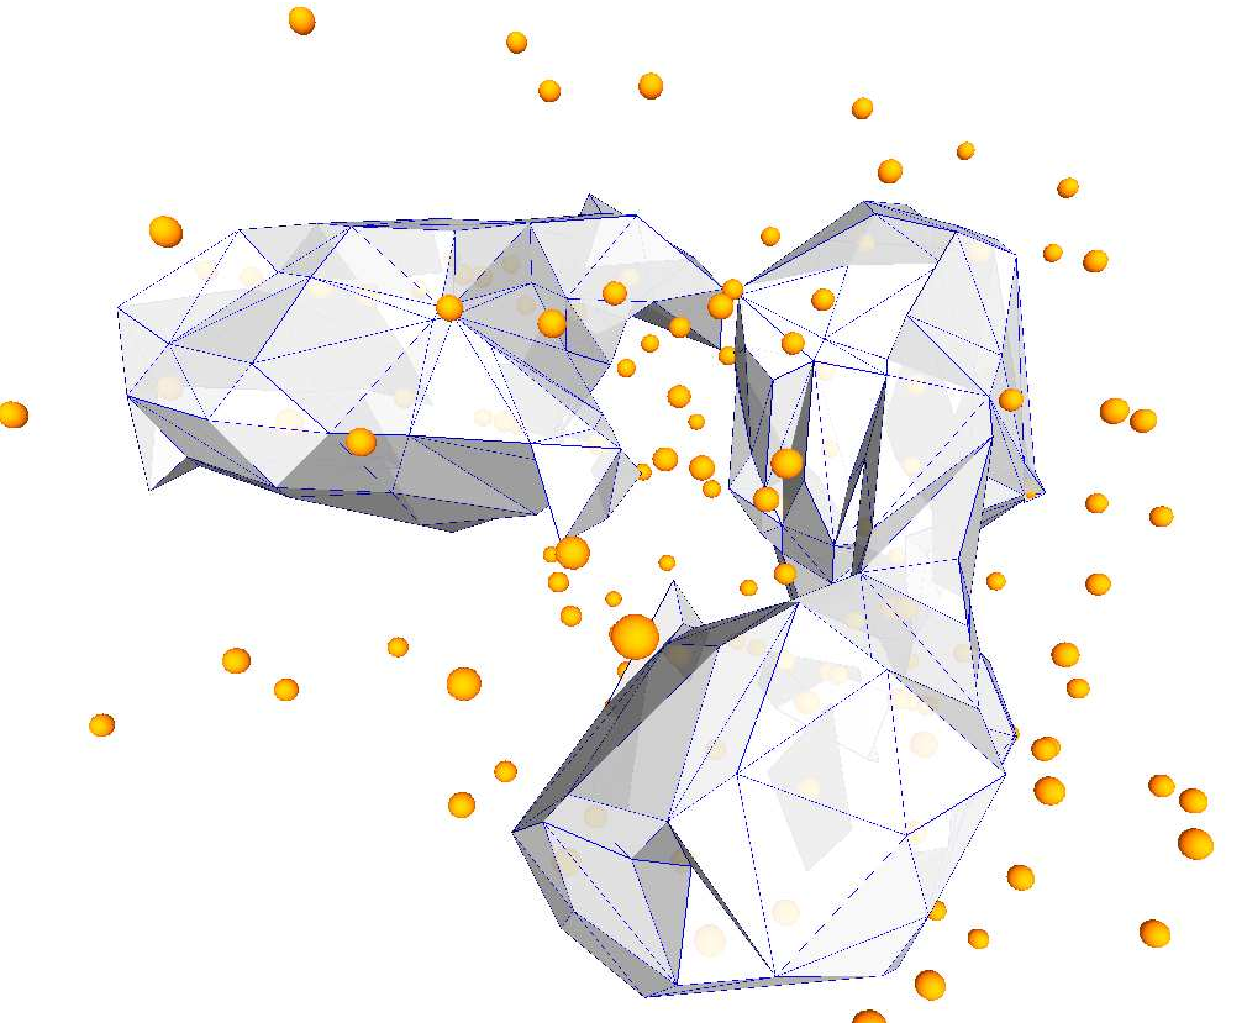
\includegraphics[width=\textwidth]{figs/isosurface25}
%     \caption{}
%   \end{subfigure}
%   \quad
%   \begin{subfigure}[b]{0.3\linewidth}
%     \centering
%     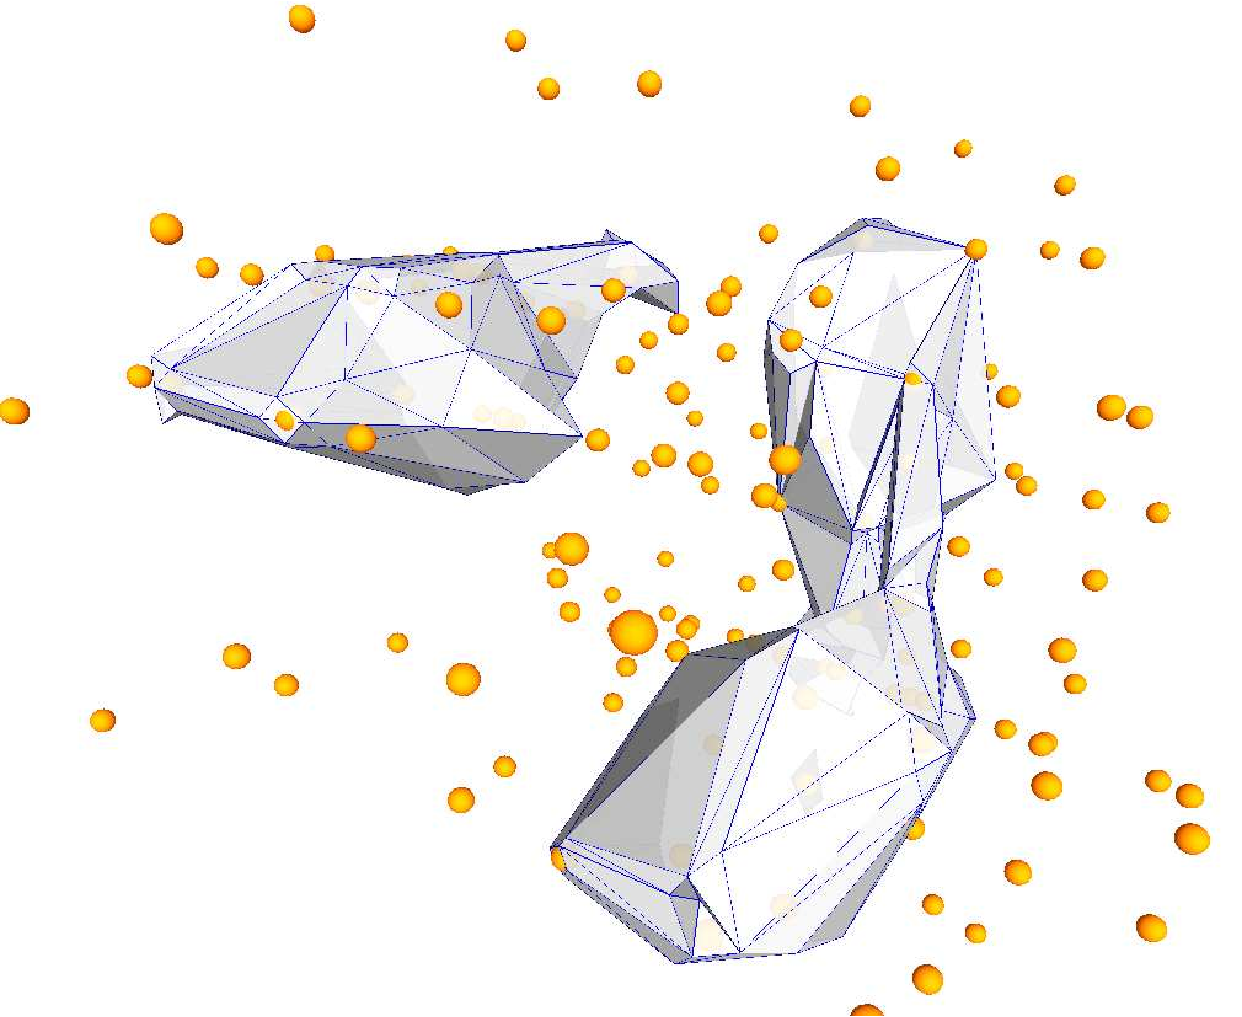
\includegraphics[width=\textwidth]{figs/isosurface3}
%     \caption{}
%   \end{subfigure}
% \caption{An example of an oceanographic dataset where each point has the temperature of the water, and three isosurface extracted (for a value of respectively 2.0, 2.5 and 3.5) from this dataset.}%
% \label{fig:isosurface}
% \end{figure*}

%

In two dimensions, isolines are usually extracted directly from a TIN or a regular grid. 
The idea is to compute the intersection between the level value (\eg\ 200m) and the terrain, represented for instance with a TIN\@. 
Each triangle is scanned and segment lines are extracted to form an approximation of an isoline.

%

In three dimensions, for a trivariate field, the same idea can be used to extract surfaces.

%

\paragraph{From a tetrahedral mesh: Marching Tetrahedra.} 
Although it is possible to fix the ambiguities, as is the case in two dimensions, the simplest solution is to subdivide each cell into simplices (cubes into tetrahedra in 3D). 
The so-called \emph{Marching Tetrahedra} algorithm is very simple: each tetrahedron is tested for the intersection with the isosurface, and triangular faces are extracted from the tetrahedra by linear interpolation on the edges. 
The resulting isosurface is guaranteed to be topologically consistent (\ie\ will not contain holes), except at the border of the dataset. 
But again, if a ``big tetrahedron''% 
\index{big tetrahedron}\marginnote{big tetrahedron}
is used where the vertices are assigned to a value lower than the minimum value of the field, then all the isosurfaces extracted are guaranteed to be `watertight'. 
The nice thing about the algorithm is that only three cases for the intersection of the isosurface and a tetrahedron can arise:
\begin{enumerate}
  \item the four vertices have a higher (or lower) value. No intersection. (Figure~\ref{fig:isosurface_3cases}a)
  \item one vertex has a higher (or lower) value, hence the three others have a lower (or higher) value. Three intersections are thus defined, and a triangular face is extracted. (Figure~\ref{fig:isosurface_3cases}b)
  \item two vertices have a higher (or lower) value and the others have a lower (or higher) value. Four intersections are thus defined. To ensure that triangular faces are extracted (better output for graphics cards), the polygon can be split into two triangles, with an arbitrary diagonal. (Figure~\ref{fig:isosurface_3cases}c)
  \end{enumerate}
\begin{figure}
  \centering
  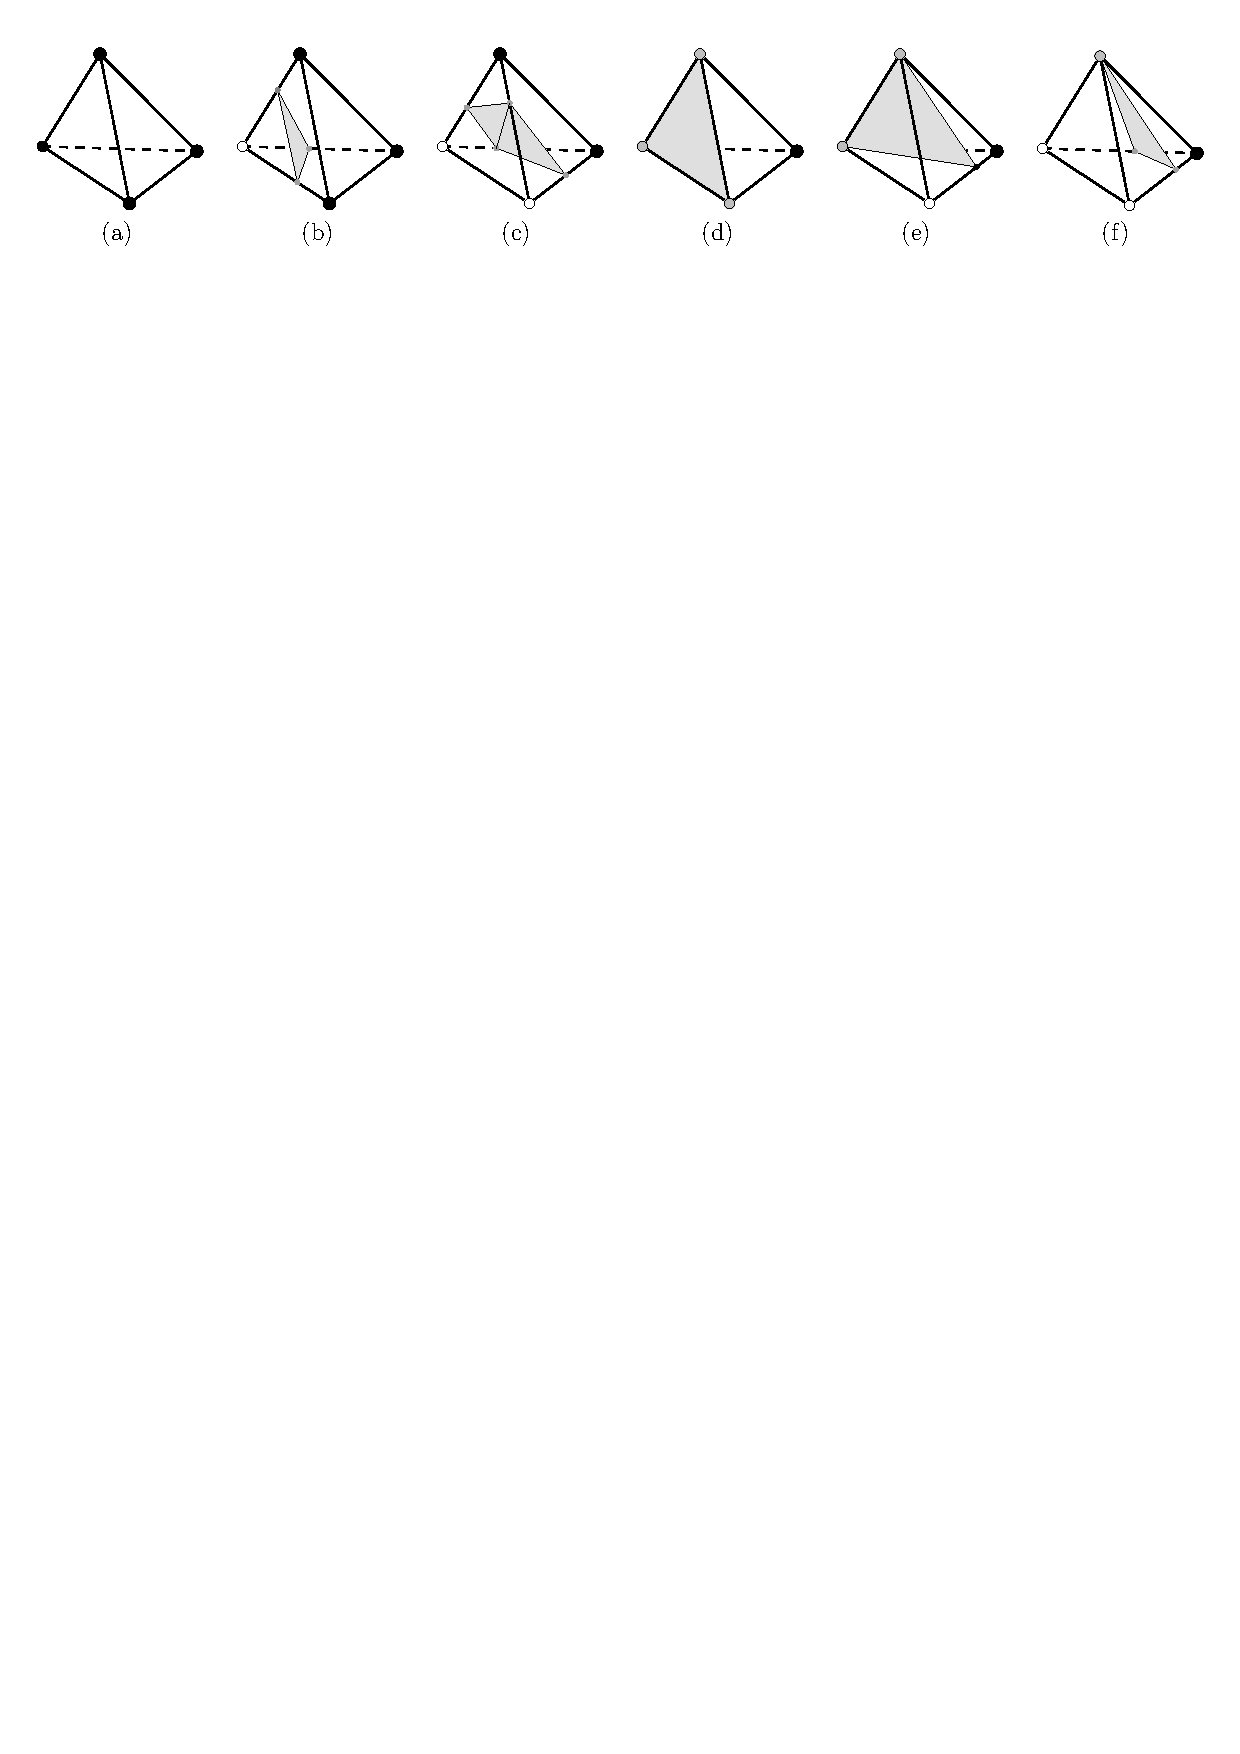
\includegraphics[width=1.0\textwidth]{figs/isosurface_3cases}
  \caption[Potential isosurface extracted for one tetrahedron]{Potential isosurface (for an attribute value $v$) extracted for one tetrahedron. Black vertex means that the attribute of this vertex is below $v$; white vertex means it is above; and grey that it is equal.}% 
\label{fig:isosurface_3cases}
\end{figure}
The only degenerate cases possible are when one or more vertices have exactly the same value as the isosurface. 
These cases are handled very easily, and the intersection is simply assumed to be at the vertices themselves (see Figure~\ref{fig:isosurface_3cases}d/e/f). 
Notice that the case when three vertices have exactly the same value, then the complete face of the tetrahedron must be extracted to ensure topological consistency.



%%%
%
\section{Conversions for objects}


%%%
% \subsection{Points to b-rep}

% In the context of the built environment, this would most likely mean that from a point cloud, a LoD2 model of the buildings, and eventually of other objects such as trees and bridges, are reconstructed. See Chapter~\ref{chap:LoD2recon}.

% It should be noticed that the b-rep can be formed solely of triangles, or of polygons.
% The polygons can have interior boundaries, as defined in ISO19107 (see Chapter~\ref{chap:iso19107}).


%%%
\subsection{b-rep to mesh}

For the purposes of this chapter, a \emph{mesh} is a collection of simplices that define the (3D) shape of an object (\eg\ a building, a tree, or a bridge).

If we take the 3D model of a building (say BK-City, see Figure~\ref{fig:bk-mesh}), 
\begin{figure}
  \centering
  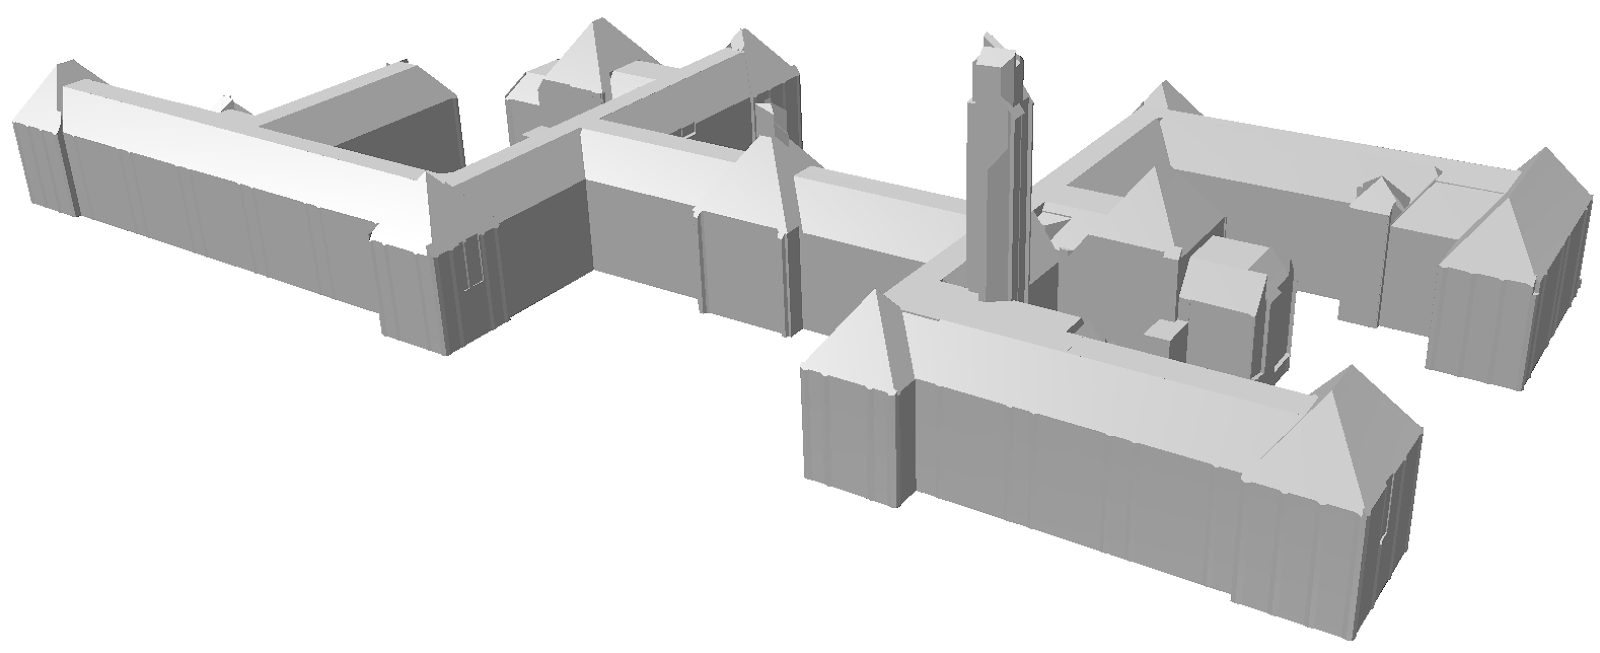
\includegraphics[width=\linewidth]{figs/bk-mesh}
  \caption{b-rep model of BK-City, from Chapter~\ref{chap:LoD2recon}}%
\label{fig:bk-mesh}
\end{figure}
this model is formed of several planar faces (hopefully) forming a closed 2-manifold.

In practice, if someone wants the mesh of this b-rep, it could mean two different structures:
\begin{description}
  \item[2D triangulation of each surface:] the constrained Delaunay triangulation, or simply an arbitrary constrained triangulation, for each of the polygon can be created. These are independently performed for each surface, and involve transforming the 3D coordinate of the vertices of the surface to a 2D system; this coordinate system is on the plane defined by the surface. Notice that this assumes that all input surfaces of the b-rep are planar, if it is not the case then finding a projection that preserves the topology of the polygon might not be possible.
  \item[Tetrahedralisation of the volume defined by the surfaces:] the cons\-trained te\-tra\-he\-dra\-li\-sa\-tion of the volume defined by the b-rep; see Chapter~\ref{chap:dtvd3d}.
\end{description}

Figure~\ref{fig:meshing} shows one example,
\begin{figure}
  \centering
  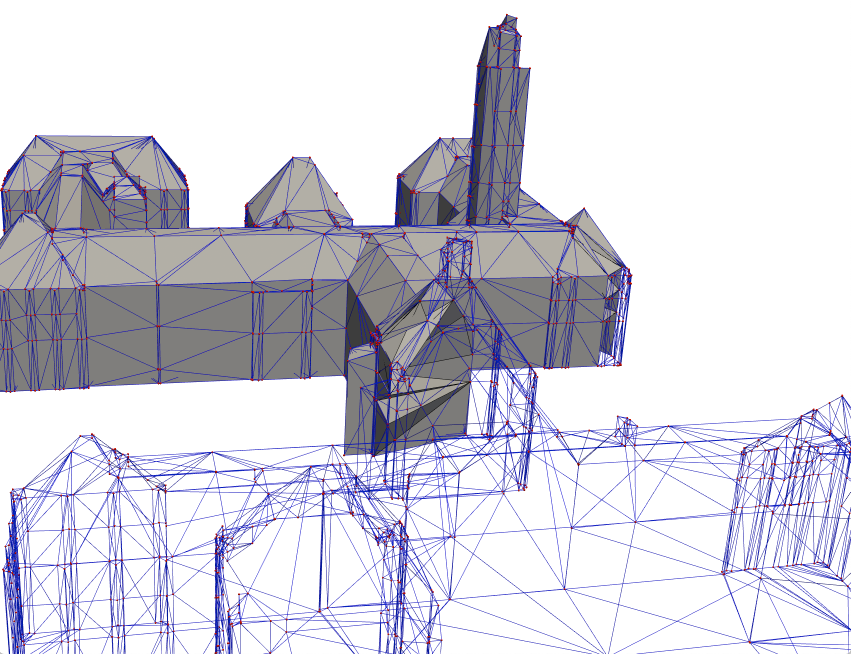
\includegraphics[width=\linewidth]{figs/mesh1}
  \caption{BK-City LoD2 b-rep tetrahedralised.}%
\label{fig:meshing}
\end{figure}
notice that the volume modelled by the boundary is tetrahedralised, but that here only some tetrahedra (in grey) are shown. 
The surfaces of the b-rep also get meshed in the same process (each surface is triangulated).


%%%
% \subsection{IFC to/from CityGML}

% The conversion between IFC (see Chapter~\ref{chap:bim}) and the CityGML data model (in either direction) is a very actual topic (many organisation would like to be able to realise it) but it is also riddled with problems caused by the differences in semantics, in data formats, and in the way geometries are modelled.
% Automatic conversion with commercial software, \eg\ FME or ArcGIS, will often ``work'', but because of the complexity of some formats, information will often be lost in the conversion. 
% Be aware.

% The following scientific paper summarises the issues and proposes one solution. 
% This solution is (mostly) based on the methods and algorithms we have studied so far in this course.

% It should be noticed that this paper is a summary of the MSc thesis of Sjors Donkers, who studied MSc Geomatics in 2014--2015.
% This MSc thesis gives you an idea of what a (very good) thesis should look like, in content and in scope.

% \begin{kaobox}[frametitle=\faExternalLink\ To read or to watch.]
%   \fullcite{Donkers16}
%   \\ \\
%   PDF: \url{https://3d.bk.tudelft.nl/hledoux/pdfs/16_tgis_ifcitygml.pdf}
%   \\ \\
%   Full MSc thesis: \url{http://resolver.tudelft.nl/uuid:31380219-f8e8-4c66-a2dc-548c3680bb8d}
% \end{kaobox}

%%%
%
\section{Notes and comments}

\citet{Cheng00} and \citet{Miller02} both describe methods to remove slivers in Delaunay meshes and to improve the shape of tetrahedra (so that they can be used for interpolation).

%%%
%
\section{Exercises}

\begin{enumerate}
  \item If the b-rep model of BK-city contains intersecting surfaces and has gaps/holes, will it be possible to mesh the model?
  \item For terrains, linear interpolation in a TIN is very popular and used. Why is it less popular for trivariate fields?
  % \item It is stated in the chapter that ``Triangulating a Voronoi cell is easily performed since it is a convex polyhedron''. Explain one method.
  % \item In the methodology of \citet{Donkers16}, why are the dilation and erosion operators used? Are they always necessary? Can you think of a simple dataset where they could be skipped?
\end{enumerate}
